\begin{figure*}[ht!]
  %
    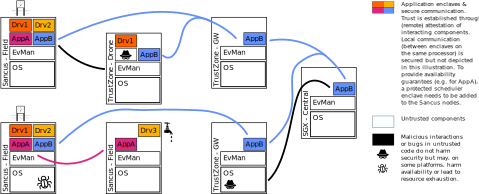
\includegraphics[height=55mm]{graphics/20210808-scenario.pdf}
  %
    \caption{A smart irrigation system as an example for distributed application
  networks we can support. Light-weight sensing and actuation nodes are deployed
  in a field. Application \emph{AppA} controls irrigation units (through driver
  \emph{Drv2}) and water supply (Drv3), based on soil moisture (obtained through
  \emph{Drv1}). Application \emph{AppB} provides similar functionality but has
  access to additional data sources, e.g., aerial surveillance and data
  aggregation on central infrastructure. All application components execute in
  enclaves (colored) and the actual composition and configuration of components
  can change dynamically. Directed data flows through untrusted networks
  (colored arrows) are at least authenticated and integrity protected;
  attestation precedes the establishment of all data flows, and mutual
  authentication is established between enclaves. All other software in the
  scenario is untrusted regarding our security properties, which leads to a very
  small run-time application \ac{TCB}. Guaranteeing availability properties may
  require a different compartmentalization strategy. The concept is also
  applicable across, e.g., the different control units within a car or in an
  autonomous robot.}
  %
    \label{fig:scenario}
  %
  \end{figure*}

\begin{figure}
  \begin{centering}
  \resizebox{0.70\linewidth}{!}{\begin{tikzpicture}
  \colorlet{cavl}{color3}
  \colorlet{cvio}{color5}
  \colorlet{csensor}{color2}
  \colorlet{cactuator}{color2}
  \colorlet{cos}{white}
  \colorlet{chw}{white}
  
  \tikzstyle{sensor}=[fill=csensor]
  \tikzstyle{actuator}=[fill=cactuator]
  \tikzstyle{os}=[fill=cos]
  \tikzstyle{avl}=[fill=cavl]
  \tikzstyle{vio}=[fill=cvio]
  \tikzstyle{eventtext}=[font=\small\ttfamily]
  \tikzstyle{event}=[->, thick, eventtext]
  \tikzstyle{evio}=[event, draw=cvio]
  \tikzstyle{eavl}=[event, draw=cavl]
  \tikzstyle{trustedhw}=[fill=chw]
  \tikzstyle{device}=[draw, thin, rounded corners, trustedhw]
  
  \newcommand{\swmodule}[3]{\node[#2] (#1) {#3}; \\}
  \newcommand{\hwnode}[4]{
    \matrix[matrix of nodes,
            draw, trustedhw,
            minimum height=80, minimum width=83,
            ampersand replacement=\&,
            nodes={draw, text width=2cm, align=center,
                   minimum height=0, minimum width=0}, #2] (#1) {
      #4
      \swmodule{}{os}{Untrusted OS}
    };
    \node[yshift=-10pt] at (#1.south) {#3};
  }
  \newcommand{\hwnodesmall}[4]{
    \matrix[matrix of nodes,
            draw, trustedhw,
            minimum height=48, minimum width=83,
            ampersand replacement=\&,
            nodes={draw, text width=2cm, align=center,
                   minimum height=0, minimum width=0}, #2] (#1) {
      #4
      \swmodule{}{os}{Untrusted OS}
    };
    \node[yshift=-10pt] at (#1.south) {#3};
  }
   
  \newcommand{\sensor}[2]{
    \draw[white] (#1) -- ++(up:20pt) coordinate (Start)
%                      -- ++(right:10pt)
                         ++(up:20pt) coordinate (Top)
%                      -- ++(10pt, -5pt)
                      -- ++(right:30pt) coordinate (End);
    \draw[thick] (#1) -- ++(up:20pt);
    \node[inner sep=0pt] at ([xshift=15pt, yshift=27pt]#1) {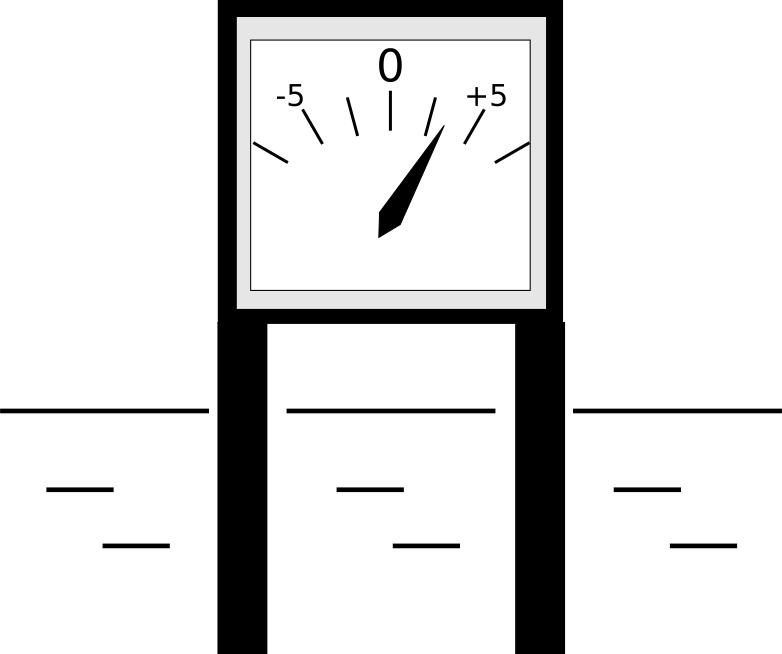
\includegraphics[width=0.08\textwidth]{graphics/clipart/moisture-meter.pdf}};
    \begin{pgfonlayer}{background}
      \node[device, fit={([yshift=-5pt]Start) (Top) (End)}, label=right:#2] {};
    \end{pgfonlayer}
  }
  
  \newcommand{\clock}[2]{
    \draw[thick] (#1) -- ++(left:15pt) coordinate (Start)
      foreach \i in {1,...,3} {
        -- ++(up:7pt) -- ++(left:5pt) -- ++(down:7pt) -- ++(left:5pt)
      } coordinate (End);
    \begin{pgfonlayer}{background}
      \node[device, fit={([yshift=-5pt]Start) ([yshift=12pt]End)}, label=#2] {};
    \end{pgfonlayer}
  }
  
  \newcommand{\display}[3]{
    \draw[thick] (#1) -- ++(right:15pt)
      node[device, anchor=west, label=#2,
           text width=50pt, align=center] (Disp-#1) {#3};
  }

  \hwnode{NP1}{}{$N_{S1}$}{
    \swmodule{SD1}{sensor}{Sensor driver}
    \swmodule{CD1}{sensor}{Clock driver}
    \swmodule{VioP1}{vio}{\module{FloS1}}
    \swmodule{AvlP1}{avl}{\module{AggS1}}
  }
  
  \sensor{SD1.165}{\dev{S1}}
  \clock{CD1.west}{\dev{T1}}
  
  \hwnode{NP2}{right=2 of NP1}{$N_{S2}$}{
    \swmodule{SD2}{sensor}{Sensor driver}
    \swmodule{CD2}{sensor}{Clock driver}
    \swmodule{VioP2}{vio}{\module{FloS2}}
    \swmodule{AvlP2}{avl}{\module{AggS2}}
  }
  
  \sensor{SD2.165}{\dev{S2}}
  \clock{CD2.west}{\dev{T2}}
  
  \hwnodesmall{NAGG}{below=of NP2}{$N_{\scriptsize\textit{Agg}}$}{
    \swmodule{Agg}{avl}{\module{Agg}}
  }
  
  \hwnode{ND1}{right=2 of NP2}{$N_{A}$}{
    \swmodule{DD1}{actuator}{Actuator driver}
    \swmodule{VioD}{vio}{\module{FloA}}
  }
  
%  \display{DD1.east}{\dev{D1}}{Violations: \\ None}
  \display{DD1.east}{\dev{A}}{Tap on/off \\
    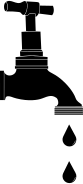
\includegraphics[width=0.25\textwidth]{graphics/clipart/tap-drops.pdf}}
  
  \hwnodesmall{ND2}{below=of ND1}{$N_{D}$}{
    \swmodule{DD2}{actuator}{Display driver}
    \swmodule{AvlD}{avl}{\module{AggD}}
  }
  
  \display{DD2.east}{\dev{D}}{Moisture: \\ 55\%}
  
  \draw[evio] (CD1.185)   -- ++(left:4pt)  |- (VioP1.west) coordinate[pos=.25] (LabelT1);
  \draw[evio] (SD1.east)  -- ++(right:6pt) |- (VioP1.5) coordinate[pos=.25] (LabelB1);
  \draw[evio] (CD2.185)   -- ++(left:4pt)  |- (VioP2.west) coordinate[pos=.25] (LabelT2);
  \draw[evio] (SD2.east)  -- ++(right:6pt) |- (VioP2.5) coordinate[pos=.25] (LabelB2);
  \draw[evio] (VioD.east) -- ++(right:6pt) |- (DD1.350) coordinate[pos=.25] (LabelD);
  
  \draw[evio, rounded corners=20pt]
      (VioP1.355)
      -- ++(right:13pt)
      -- ++(20pt, 70pt)
      to[bend left] node[above]{Flooded} ++(right:130pt)
      -- ++(20pt, -50pt)
      --   (VioD.175);
  \draw[evio] (VioP2.355) to[bend right=10] node[below] {Flooded} (VioD.185);
  
  \draw[eavl] (SD1.west)  -- ++(left:6pt) |- (AvlP1.west);
  \draw[eavl] (SD2.west)  -- ++(left:6pt) |- (AvlP2.175);
  \draw[eavl] (AvlD.east) -- ++(right:6pt) |- (DD2.350) coordinate[pos=.25] (LabelD2);

  \draw[eavl] (AvlP1.east) to[out=0,   in=180]                coordinate (LabelM1) (Agg.185);
  \draw[eavl] (AvlP2.185)  to[out=180, in=180, looseness=0.7] coordinate (LabelM2) (Agg.175);
  \draw[eavl] (Agg.east)   to[bend right=10]                  node[below,
eventtext] {MoistChanged} (AvlD.west);

  \begin{scope}[inner sep=0, eventtext]
    \draw (LabelD)  to[bend left]  ++(10pt, -10pt)
                                   node[below right] {Tap};
    \draw (LabelD2)  to[bend left]  ++(10pt, -10pt)
                                   node[below right] {Display};
    \draw (LabelB1) to[bend left]  ++(10pt, 10pt)
                                   node[below right, rotate=90] {Sensor};
    \draw (LabelB2) to[bend left]  ++(10pt, 10pt)
                                   node[below right, rotate=90,
xshift=-25pt] {Sensor};
    \draw (LabelT1) to[bend right] ++(-10pt, -10pt)
                                   node[below left] {Tick};
    \draw (LabelT2) to[bend right] ++(-10pt, -10pt)
                                   node[below left] {Tick};
    \draw (LabelM2) to[bend right] ++(-8pt, 8pt)
                                   node[above, rotate=90] (CarMoved) {Moisture};
    \draw (LabelM1) to[bend left] (CarMoved.north);
  \end{scope}
\end{tikzpicture}
}
  \end{centering}
  \vspace{-3mm}
  \caption{%
    Our running example with two applications, \appavl{} (\coloriiiname{}) and
\appvio{} (\colorvname{}). Hardware ($N_{*}$ and $D_{*}$) is trusted; the OS and
the network are untrusted. E.g., the \appvio{} deployer creates the three
\colorvname{} \acp{SM} (cf. \cref{code:appvio}) with a trusted compiler, attests
the shared sensor-, clock- and display drivers and sets-up connections between
the \acp{SM}. Remote attestation assures authentic execution of \appavl{} and
\appvio{}. } %
  \label{fig_model}
  \vspace{-3mm}
\end{figure}



\section{Running Example, Infrastructure \& Objectives}
\label{sec:system}

As a running example we discuss an automated irrigation system, as illustrated
in Figure~\ref{fig:scenario}, which involves a series of light-weight sensors
and actuators in the field that, e.g., monitor soil moisture and crop growth,
and control water supply. The system can be connected to edge infrastructure or
cloud services for centralized configuration and maintenance, to integrate
reporting and billing, and to minimize water consumption based on weather
predictions. Naturally, smart farming systems are security critical since
malicious interactions can potentially lead to huge costs and may destroy a
crop; they also feature a high level of dynamicity where equipment needs to be
reconfigured for specific sensing and actuation tasks that depend on the type of
crop~\cite{raghavan_computational_2016} and, e.g., sustainability
objectives~\cite{streed_how_2021}, and demand a high level of dependability
where events must be guaranteed to be processed in a timely manner.

\Cref{fig_model} (source code in \cref{code:examples}) zooms in on the
light-weight in-field sensing and actuation on the left side in
\cref{fig:scenario} and details application modules and event flows in an
agricultural sensor network with two soil moisture sensors. The infrastructure
can be reused for multiple applications which can be provided by different
stakeholders. Applications include visualizing soil moisture, targeted
irrigation, or detection of flooding or leakage. We show two of these
applications: one (\appvio) that detects flooding or leakage and disconnects the
water supply in case of emergency, and another (\appavl) that aggregates and
displays data on soil moisture.

\subsection{The Shared Infrastructure}
\label{concept:shared-infrastructure}
\label{concept:nodes}
%
The infrastructure is a collection of \emph{nodes} ($\node{i}$), where each node
consists of a processor, memory, and a number of \emph{I/O devices} (\dev{i}).
Multiple mutually distrusting stakeholders share the infrastructure to execute
distributed \emph{applications} ($\app{i}$). For simplicity, we assume
processors are simple microprocessors, such as the OpenMSP430 used in our
prototype, to explain the underlying concepts and security guarantees of our
approach. As we detail in Section \ref{sec:implementation} and thereafter, our
implementation does support the commercial \acp{TEE} TrustZone and Intel
\ac{SGX}, and we evaluate our approach on an integrated scenario that involves
these \acp{TEE}.
 
An I/O device interfaces the processor with the physical world and
facilitates
\begin{paraenum}
  \item sensing physical quantities (e.g., the state of a switch),
  \item influencing physical quantities (e.g., an LED), and
  \item notifying the processor of state change (e.g., a key being pressed) by
  issuing an interrupt.
\end{paraenum}

In our running example there are 5 nodes. Two of these (\node{S1} and \node{S2})
are each attached to two input devices (a clock \dev{Ti} and a soil moisture
sensor \dev{Si}), and are installed in a field, e.g., along a row of crops. Two
other nodes (\node{A} and \node{D}) are connected to actuator and display
devices (\dev{A}, \dev{D}) to control the water supply and show application
output. One node (\node{\textit{Agg}}) is not connected to any I/O device but
performs general-purpose computations, e.g., aggregate data from sensor nodes.

\begin{figure}[ht]
  \begin{centering}
  \hfill
  \subfloat[\appvio]{
    \parbox{.4\linewidth}{\lstinputlisting[language=Reactive]{appflo.reactive}}
    \label{code:appvio}
    \vspace{-2mm}
  }
  \hfill
  \subfloat[\appavl]{
    \parbox{.4\linewidth}{\lstinputlisting[language=Reactive]{appagg.reactive}}
    \label{code:appavl}
    \vspace{-2mm}
  }
  \hfill\mbox{}
    \vspace{-2mm}
  \caption{ Pseudo-code of the applications from \cref{fig_model}. in a
    Python-like syntax. Enclaved application components are declared using the
    \code{module} keyword and span until the next \code{module} or the end of
    the file. The \code{on} statement starts an event handler which can connect
    to an output of another application component, or to a physical I/O channel.
    Outputs are implicitly declared when invoked through a function call-like
    syntax. }
  \label{code:examples}
  \end{centering}
  \vspace{-3mm}
\end{figure}


\subsection{Modules \& Applications}
%
We use an event-driven application model and \emph{modules} (\module{i}) contain
input- and output channels. Upon reception of an event on an input channel, the
corresponding event handler is executed atomically and new events on the
module's output channels may be produced.

An application, then, is a collection of modules together with a
\emph{deployment descriptor}. This descriptor specifies on which nodes the
modules should be installed as well as how the modules' channels should be
connected. Channels can be connected in two ways. First, one module's output
channel can be connected to another's input channel, behaving like a buffered
queue of events. Second, the infrastructure can provide a number of
\emph{physical} I/O channels which can be connected to a module's I/O channels.
\label{concept:physical-io-channel}
The infrastructure must ensure that events on such channels correspond to
physical events: An event received on a physical input could correspond to a
button press or, similarly, an event produced on a physical output could turn on
an LED. An important contribution of this paper is a design to securely connect
modules to physical I/O channels
(\cref{concept:protected-drivers,concept:secure-io-sancus}).

In our example applications (\cref{fig_model}), \appvio{} consists of three
modules: two (\module{\textit{FloS1}} and \module{\textit{FloS2}}) are deployed
in a field and detect excess moisture (flooding or leakage) and one
(\module{\textit{FloA}}) actuates a central tap to disconnect water supply if
needed. The two in-field modules have two inputs that are connected to input
devices provided by the infrastructure: one that produces events for changes in
soil moisture (\dev{Si}) and another that sends periodical timer events
(\dev{Ti}). As the source code (\cref{code:appvio}) shows, these modules first
wait for changes in critical changes in soil moisture, then wait for a maximum
number of timer events, and finally produce an output event to indicate an
emergency. These output events are connected to the inputs of
\module{\textit{FloA}} which in turn produces output events  and sends them to
the output actuator \dev{A}. A second application \appavl{} shares access to the
sensor drivers with \appvio{} to obtain sensor readings that are then aggregated
and displayed.

\subsection{Attacker Model}
\label{concept:attacker}
%
We consider powerful attackers that can manipulate all the software on the
nodes. Attackers can deploy their own applications on the infrastructure, but
they can also tamper with the OS. Attackers can also control the communication
network that nodes use to communicate with each other. Attackers can sniff the
network, modify traffic, or mount man-in-the-middle attacks. With respect to the
cryptographic capabilities of the attacker, we follow the Dolev-Yao
model~\cite{dolev-yao}.

Attacks against the hardware are out of
scope. We assume the attacker to not have
physical access to the nodes, neither can they physically tamper with I/O
devices. We also do not consider side-channel attacks against our
implementation. Physical protection and side-channel resistance are important
but orthogonal and complementary to the protection offered by our approach.

\subsection{Security Objective}
\label{concept:goals}
\label{concept:deployer-tcb}

The deployer uses his own (trusted) computing infrastructure to compile the
application $A$, to deploy the modules to the nodes in the shared
infrastructure, and to configure connections between modules, and between
modules and physical I/O channels. At run-time, a sequence of physical input
events will happen, and the deployer can observe the sequence of physical output
events that return. We say that this sequence of outputs is \emph{authentic} for
an application $A$ if it is allowed by $A$'s modules and deployment descriptor
in response to the actual trace of input events: the source code of $A$ explains
the physical outputs on the basis of actual physical inputs that have happened.
\Cref{concept:deployment} will detail this sequence of physical input,
processing, and lastly physical output further.

Our objective is to design a deployment algorithm such that the deployer can
easily certify the authenticity of sequences. If the correctness of the
deployment is verified, then our approach guarantees that any subsequent trace
of output events observed by the deployer will be authentic.
%
This security notion rules out a wide range of attacks, including attacks where
event transmissions on the network are spoofed or reordered, and attacks where
malicious software tampers with the execution of modules. Other relevant attacks
are \emph{not} covered by this security objective. We will explain more nuances
regarding deployment in \cref{concept:deployment}.

As discussed earlier, there are no general availability guarantees -- e.g., the
attacker can suppress network communication. However, \ac{TEE} extensions such
as~\cite{alder_2021_aion} and the use of real-time operating systems can provide
notions of availability that are relevant to maintain system safety in, e.g.,
autonomous control systems. There are also no strong confidentiality guarantees:
Although this is not the focus of our design, our implementation \emph{does}
provide substantial protection of the confidentiality of application state as
well as event payloads. Yet, the attacker may still observe the occurrence and
timing of events in the system, and specifically on the sensing-and-actuation
side of our systems, this information may very well reveal the state of the
system. While it is technically possible to close these side channels, e.g.,
with artificially generated noise, this is infeasible for our light-weight
\acp{TEE} and under constrained energy consumption (cf.
\cref{sec:discussion:confidentiality} for details).

Many systems similar to our running example from Figure~\ref{fig:scenario}
exist, e.g., in the context of the Internet of Things, smart building, supply
chain management, or intelligent transport systems. These may come with
different requirements regarding security and privacy, potentially beyond the
baseline guarantees of our framework. In Section~\ref{eval:intro} we look
specifically at a smart-home scenario and discuss performance characteristics
and security guarantees (cf. Section~\ref{sec:discussion}).
